


\subsection{Pair-acceptance correction with event mixing}
\label{sec:EventMixing}
Event mixing is a data driven approach to correcting for detector acceptance effects and estimating combinatorial background. By constructing observables with particles from different events, we remove true physics correlations from the correlation functions, isolating detector effects from limited acceptance in \(\eta\) and detector inhomogeneity in $\eta$ and $\varphi$. 

We mix events which are as similar as possible. To this end, events are often classified by multiplicity (V0 amplitude, sum of V0A and V0C) and primary vertex $z$-position bins, and then mixed within these bins. The mixing in this analysis was carried out using a Gale Shapely matching algorithm~\cite{GaleShapley:1962amm}. The use of this algorithm avoids the need for binning in multiplicity and primary vertex.

Instead of bins, events are split into blocks of 2000. For each event in the block, the multiplicity and z-vertex position are compared between all other events in the block. The algorithm then creates a preference list containing all other events in the block for each event based on how close events are in multiplicity and $z$-vertex. In order for the mixed event distribution to reflect background instead of emulating  signal, as well as to fully cover the detector acceptance, we paired each \(\gamma\)-triggered event with minimum bias events. Subsequent batches of 200 minimum bias events are used, as necessary, to reach the desired number of mixed events per true event. For this analysis, depending on the \zt~bin, each \(\gamma\)-triggered event was mixed with up to 300 minimum-bias events. 

After each event has an associated preference list, the algorithm loops through all events in the block, and then loops through each event's associated preference list to pair it to the first unpaired event on that list. As the loop iterates, if an event towards the end of the main loop has an already-paired event high on it’s preference list, the algorithm loops through the already-paired event's preference list and decides if the paired event should stay paired to its current match, or switch to the new event. If the latter is chosen, the previously matched event is “unpaired” and added back into the loop. A stable state is met when all paired events have a match that is higher on their preference list than any remaining unpaired events in the loop. Such a stable state is guaranteed to eventually be met according to Ref.~\cite{GaleShapley:1962amm}.

The pseudo code below follows this description, using \(\gamma\) to denote a \(\gamma\)-triggered event, and \(M_B\) to denote a minimum-bias event. The \textit{unrequested} state refers to a \(M_B\) event on a \(\gamma\)-event's preference list that has not yet been requested for pairing.\\

\FloatBarrier
\begin{algorithmic}
\Procedure{GaleShapleyPairing}{}
\While{\(\exists\) \textit{free} \(\gamma\) with an unrequested \(M_B\) on \(\gamma\)'s list}
\State \(M_B\) = first unrequested MinBias Event on \(\gamma\)'s list.
\If {\(M_B\) is free}
\State (\(\gamma\),\(M_B\)) become paired
\Else{ some pair (\(\gamma\)',\(M_B\)) exists}%
	\If{\(M_B\) prefers \(\gamma\) to \(\gamma\)'}
    \State \(\gamma\)' becomes free
    \State (\(\gamma\),\(M_B\)) become paired
    \Else
    \State (\(\gamma\)',\(M_B\)) remain paired
    \EndIf
\EndIf
\EndWhile
\EndProcedure
\end{algorithmic}

\begin{figure}[h]
\center
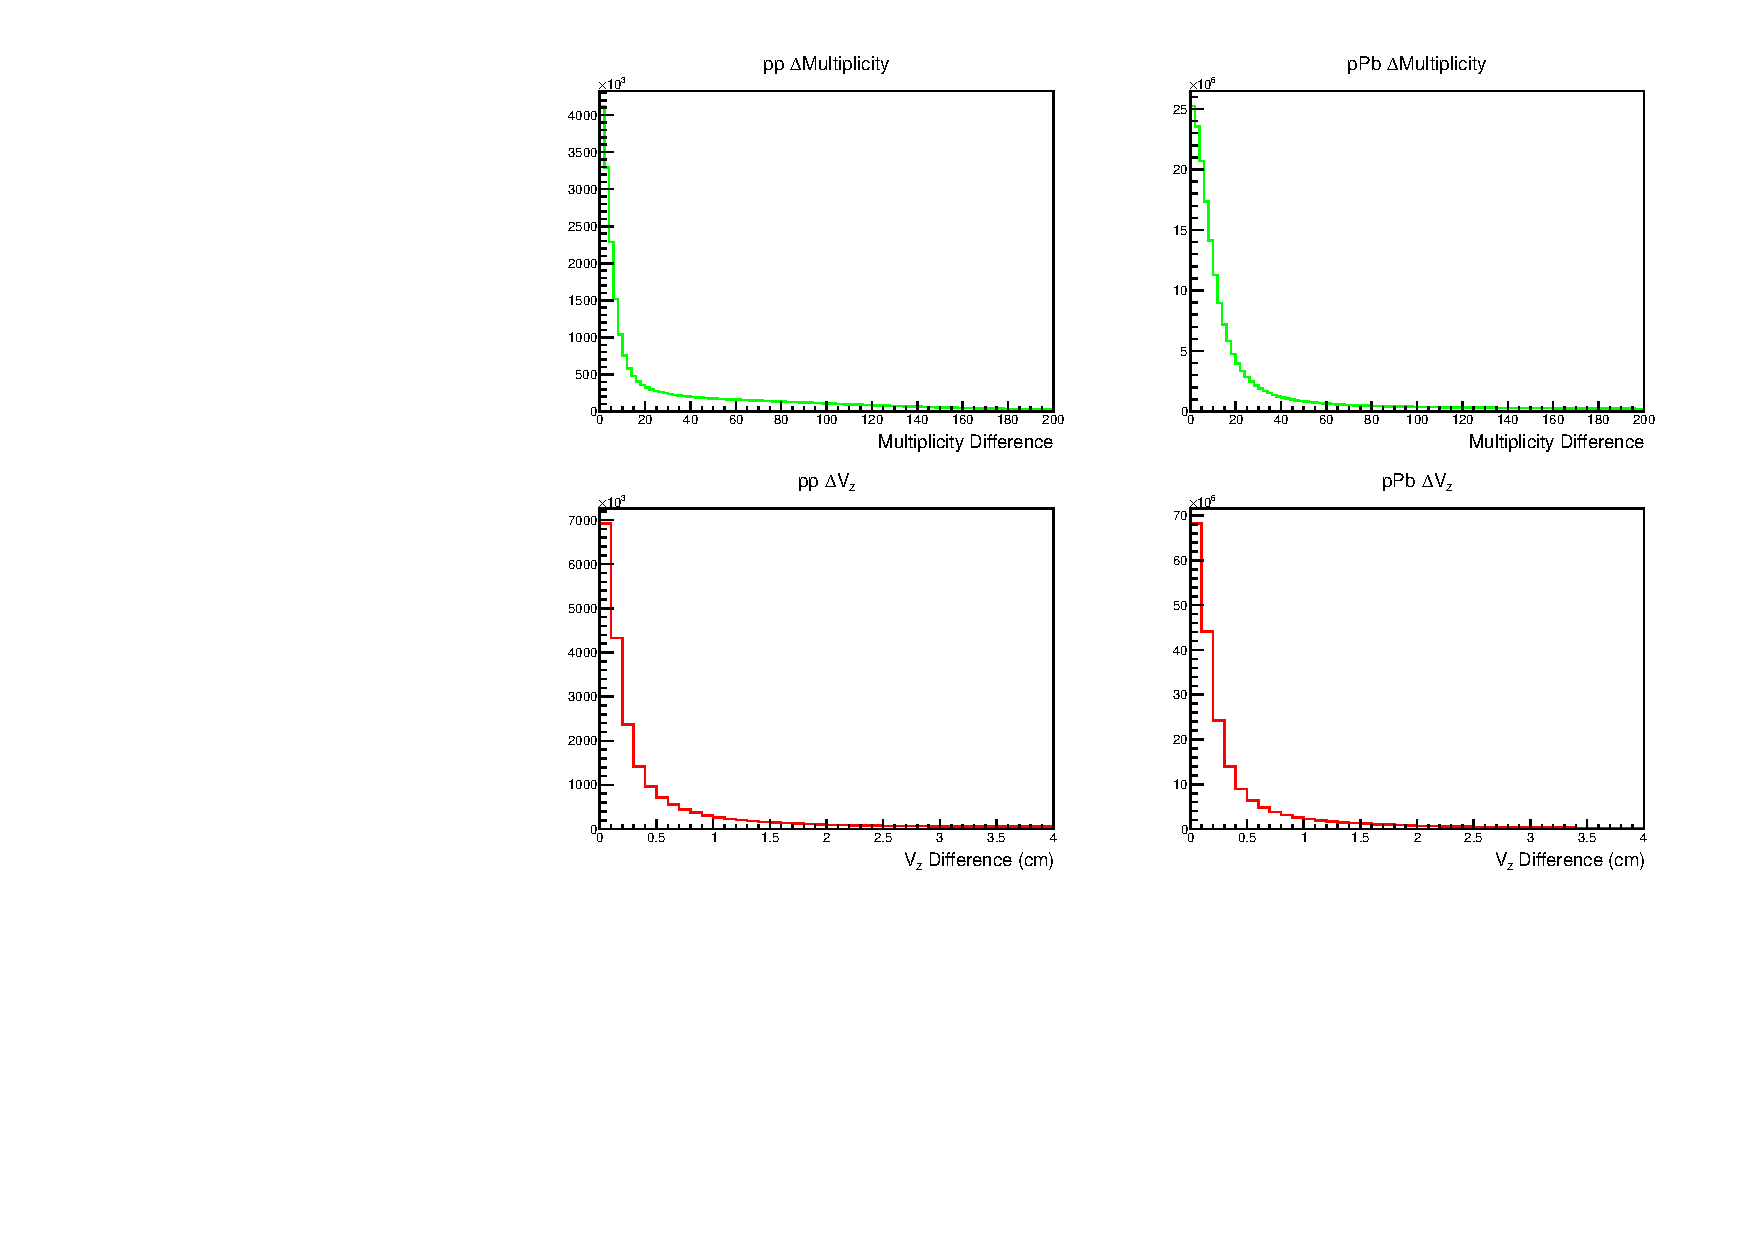
\includegraphics[width=0.95\textwidth]{EventMixing/pPb_Differences.pdf}
\caption{Difference in V0 multiplicity
(upper row) and longitudinal vertex position (bottom row) between paired events in pp (left column) and \pPb~right. The pairing algorithm results in sharp peak near zero for these difference distributions, particularly in the longitudinal vertex difference. As described in the text, in the correlation analysis we apply a further selection to cut the large tails observed in these distributions. }
\label{Difference_distributions}
\end{figure}

The difference distributions for Z-vertex and multiplicity between a \(\gamma\)-triggerd and minimum bias events in \pPb~data are shown in Figure \ref{Difference_distributions}. The resulting distributions show a sharp peak that is below {$\Delta z<0.5$ cm} and also a long tail. Less than 6 \% of the distribution lies beyond $\Delta z > 2$ cm. The multiplicity difference, however, does not have as sharp a peak near \(\Delta\)Multiplicity = 0. About 20$\%$ of pairs have a multiplicity difference above 40, and cuts at \(\Delta V_z > 2\)cm and \(\Delta\)Multiplicity \(> 40\) were applied to pairs before calculating correlation functions.

Figure~\ref{fig:Multiplicitydistributions} shows the V0 multiplicity distributions for pp and \pPb~data in $\gamma$--triggered events. This shows that a multiplicity matching requirement of \(\Delta\)Multiplicity \(< 40\) is indeed very tight. 

\begin{figure}[h]
\center
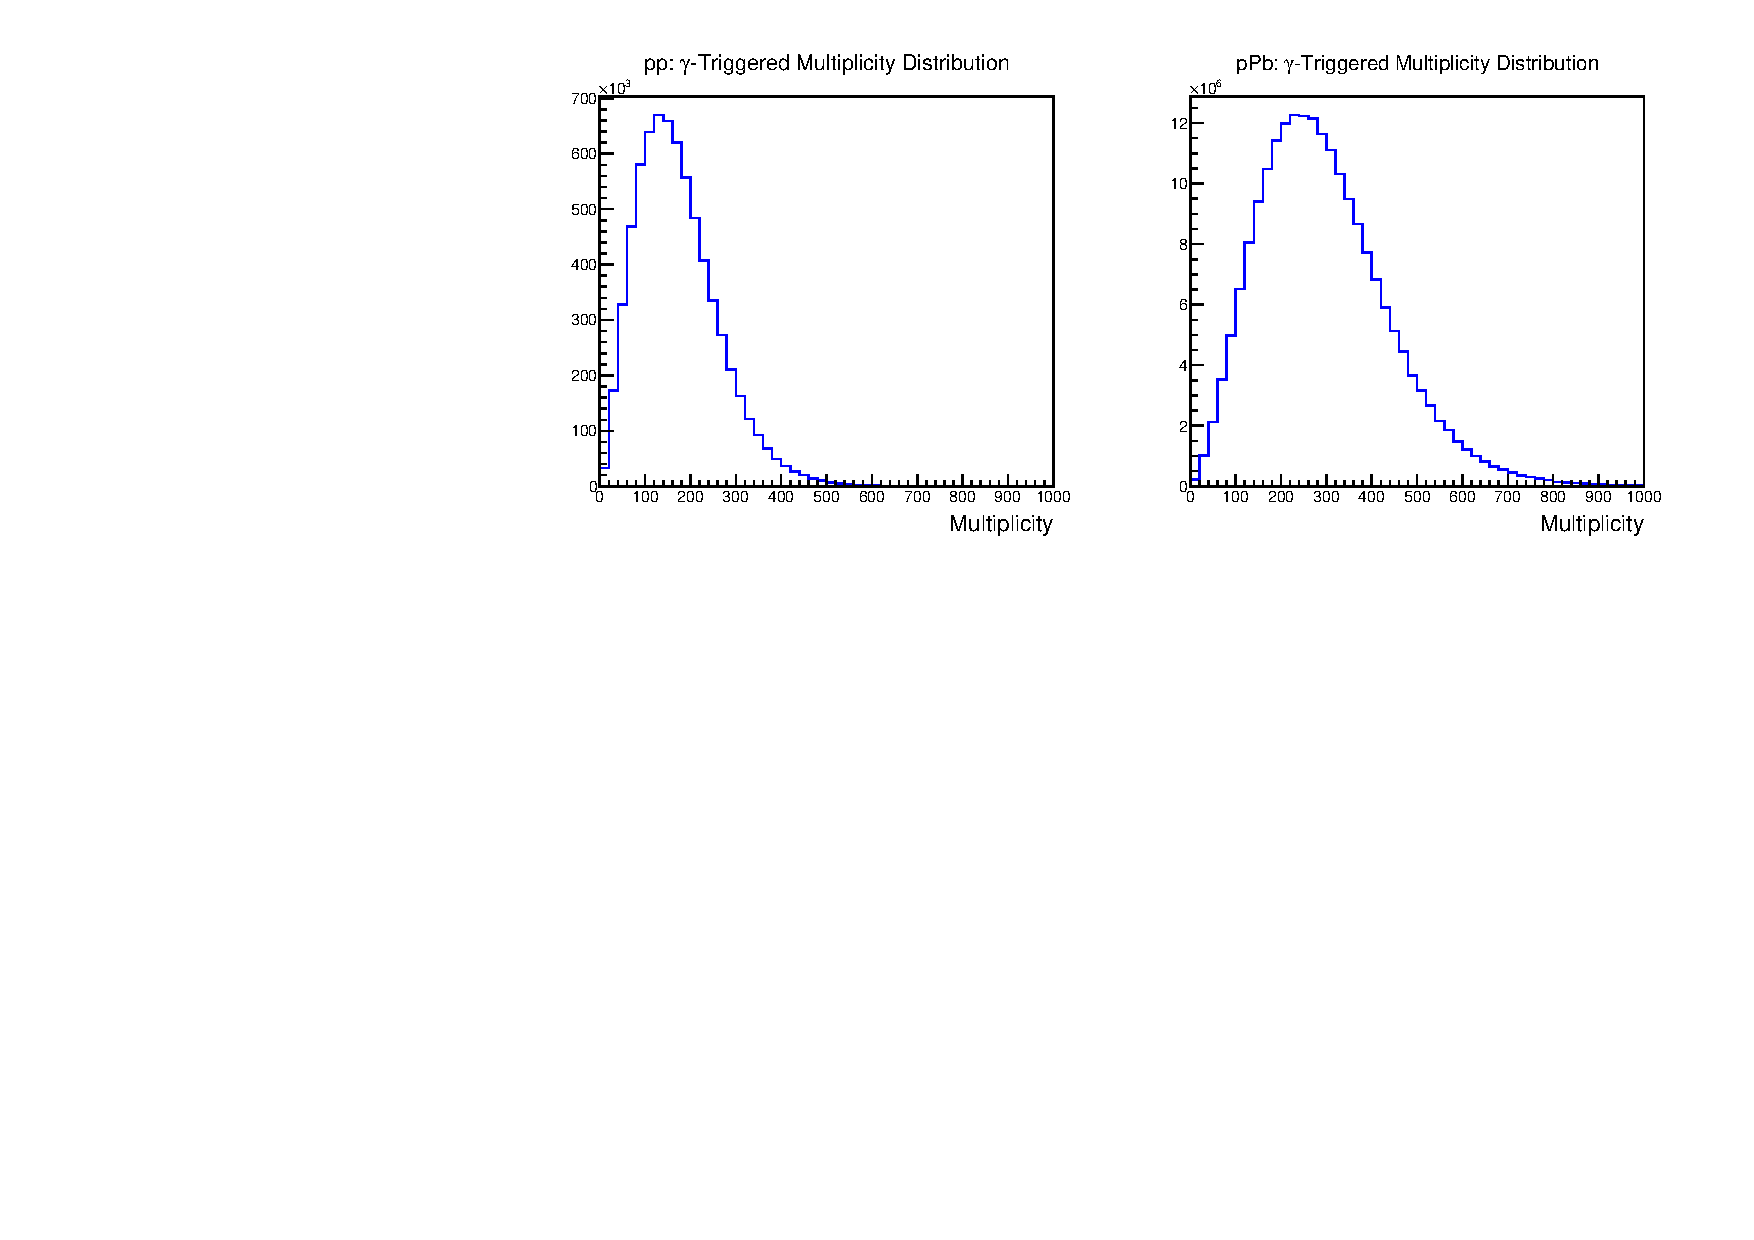
\includegraphics[width=0.9\textwidth]{EventMixing/Abs_Multplicity_Dist.pdf}
\caption{V0 multiplicity distribution, i.e. the sum of V0A and V0C amplitudes , in pp (left) and \pPb~(right) gamma-triggered data.}
\label{fig:Multiplicitydistributions}
\end{figure}

Ideally, the mixed event distribution should be flat in \(\Delta\varphi\) and have a trapezoidal shape in \(\Delta\eta\), because the limited acceptance in \(\eta\) increases the likelihood to reconstruct pairs with a small \(\Delta\eta\) (i.e, due to the convolution of two uniformly distributed functions). However, the use of ITS-only tracks and holes in the ITS acceptance result in deviations from a flat distribution in \(\Delta\varphi\). %This is visible in Figure~\ref{GS_Mixed_2D}.

%The highest efficiency to find pairs between the ITS and EMCal should be equal to unity. Thus, the normalization was chosen such that the maximum value of the correction is equal to unity. 
The correlation function corrected by pair-acceptance effects is then given by:

\begin{equation}
\label{eq:Y}
C(\Delta \varphi, \Delta \eta) = \frac{S(\Delta \varphi, \Delta \eta)}{M(\Delta \varphi, \Delta \eta)}
\end{equation}, 

where $S(\Delta \varphi, \Delta \eta)$ is the same-event correlation, and $M(\Delta \phi, \Delta \eta)$ is the mixed-event correlation. $S(\Delta \phi, \Delta \eta)$ is given by: 
\begin{equation}
S(\Delta \varphi, \Delta \eta) = \frac{1}{N_{\mathrm{trig}}}\frac{d^2N_{\mathrm{same}}}{d\Delta \varphi d\Delta \eta}
\end{equation}

With \Ntrig~as the number of trigger particles and \Nsame~as the number of same event cluster-track pairs and $d^2\Nsame/d\Delta \varphi d\Delta \eta$ is found by pairing trigger particles with tracks from the same event. The mixed-event distribution, $M(\Delta \varphi, \Delta \eta)$, is given by 
\begin{equation}
M(\Delta \varphi, \Delta \eta) = \alpha \frac{d^2 \Nmixed}{d\Delta \varphi d\Delta \eta}.
\end{equation}

Where $\alpha$ is the normalization constant that sets the maximum value of the mixed event correlation to 1, and \Nmixed~is the number of mixed event cluster-track pairs. The term $d^2 \Nmixed/d\Delta \varphi d\Delta \eta$ is obtained by pairing trigger particles from \(\gamma\)-triggered events with tracks from minimum bias events matched in z-vertex and multiplicity.


\begin{figure}
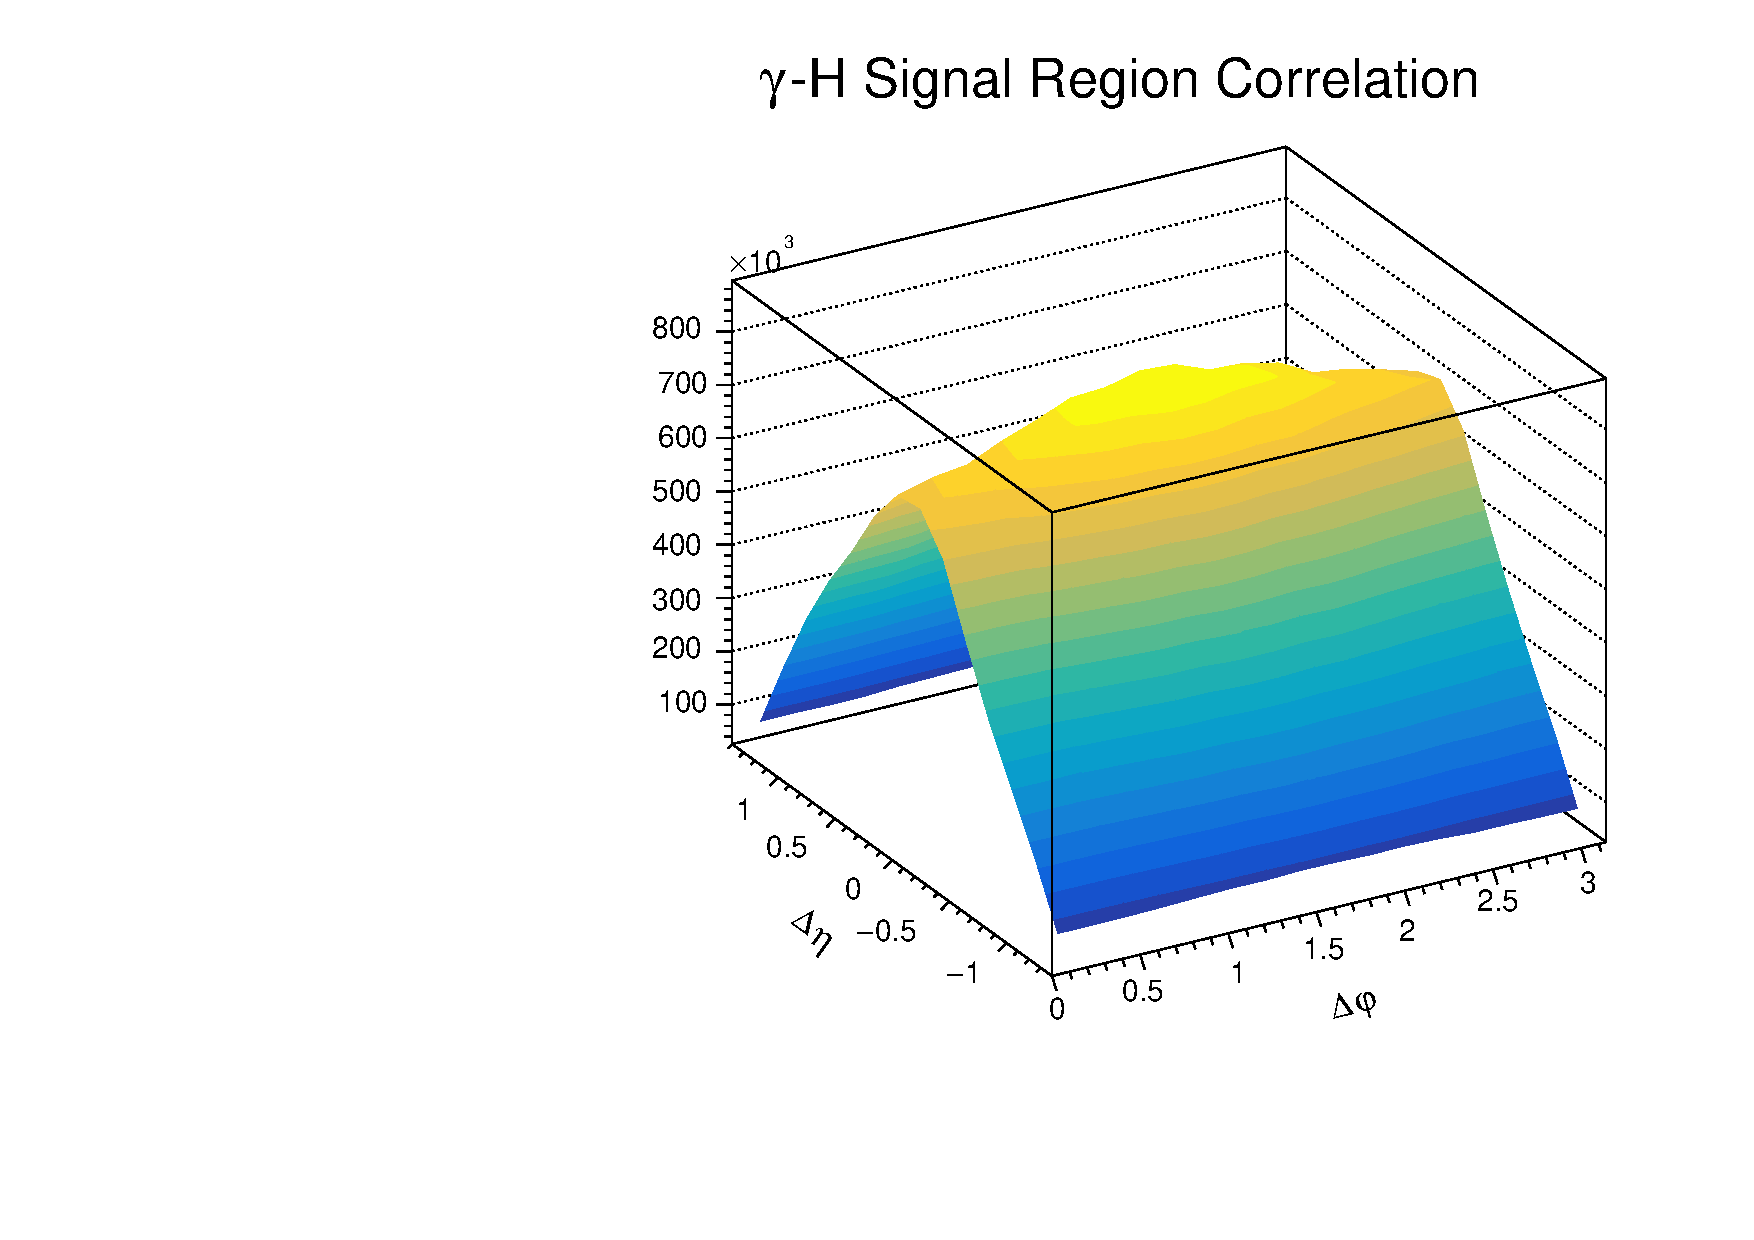
\includegraphics[width=0.32\textwidth]{G-H_New/2D_SR_ME.pdf}
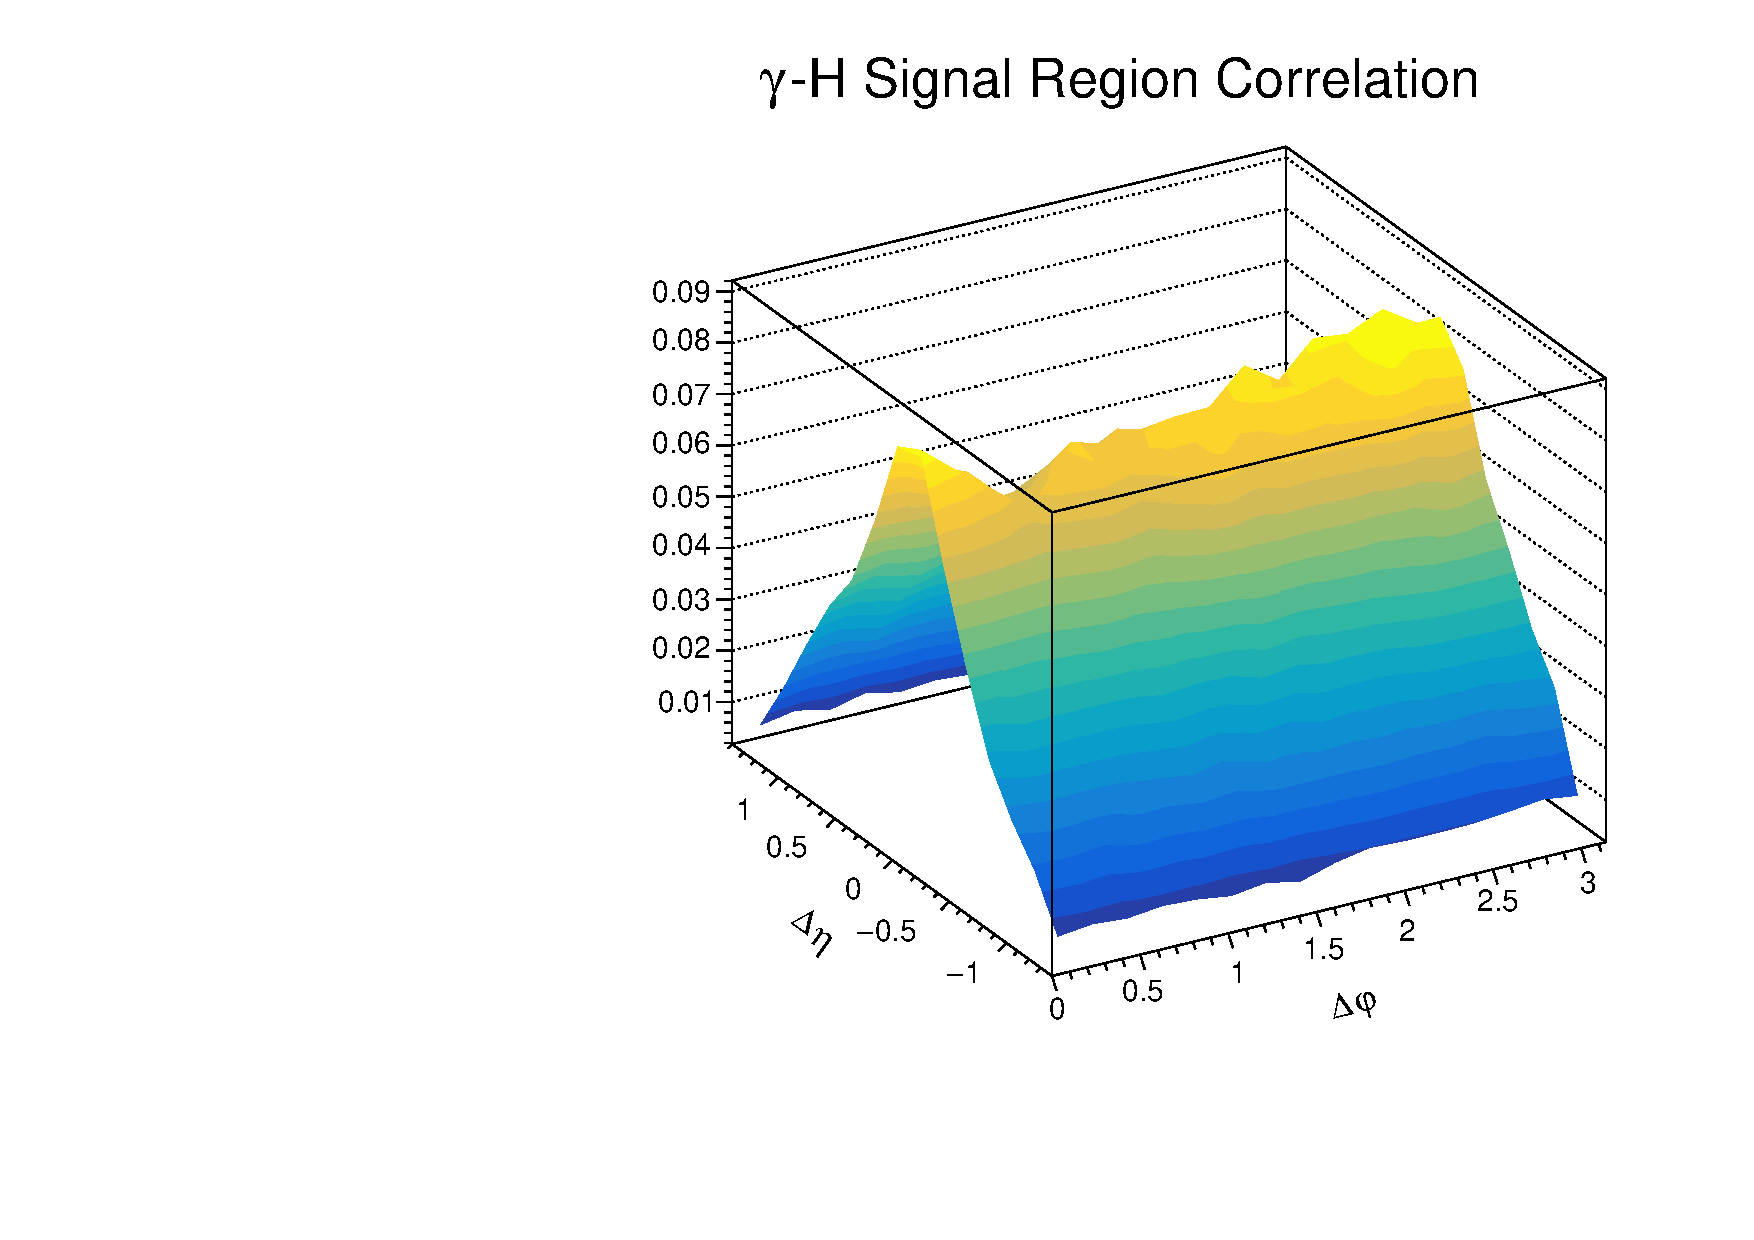
\includegraphics[width=0.32\textwidth]{G-H_New/2D_SR_SE.pdf}
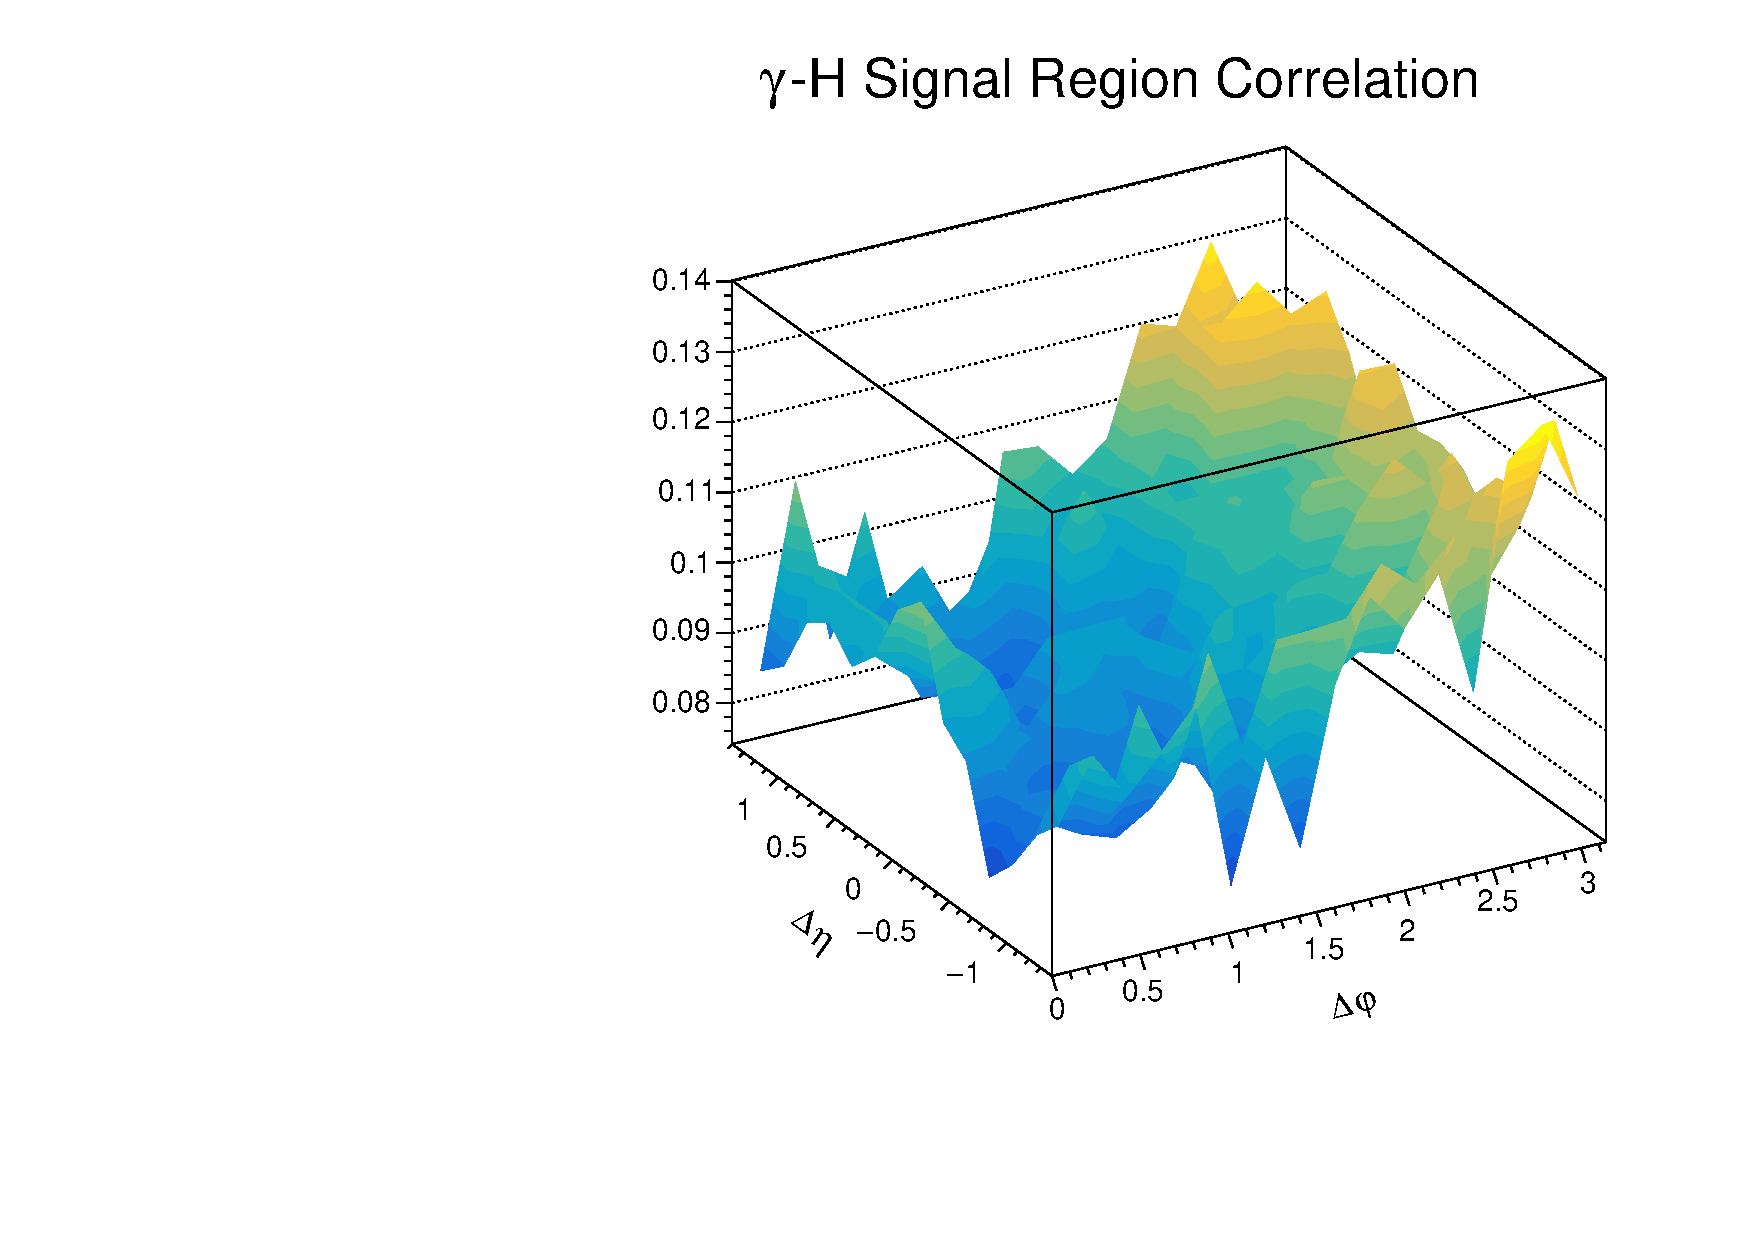
\includegraphics[width = 0.32 \textwidth]{G-H_New/2D_SR.pdf}
\caption{\textbf{Left} Mixed Event correlation for a single \zt~bin for gamma-triggered, signal region clusters and hadrons from minimum bias events. \textbf{Middle} 2D Correlation for signal region clusters and hadrons from the same events. \textbf{Right} Signal region correlation function corrected for detector acceptance effects.}
\label{fig:SR_2D}
\end{figure}

Same event correlation functions were divided by the mixed event correlation function within the same \zt~bins, shown for a single \zt~bin in Figure~\ref{fig:SR_2D}. This procedure is carried out identically for clusters in the signal and background shower-shape regions. 




%Thus, $Y(\Delta \phi, \Delta \eta)$ in equation \ref{eq:Y} relates to $C_{\mathrm{SR}}$ and $C_{\mathrm{BR}}$ from equation \ref{eq:CSRCBR} in the following way:

%\begin{eqnarray}
%Y_S(\Delta \varphi, \Delta \eta) &=& C_{\mathrm{SR}}\\
%Y_B(\Delta \varphi, \Delta \eta) &=& C_{\mathrm{BR}}
%\end{eqnarray}

%Where $Y_{\mathrm{S}}$ is the overall yield per trigger isolated, single  photon correlation %function, and $Y_{\mathrm{B}}$ is the overall yield per trigger isolated  merged cluster correlation function.

%\begin{figure}
%\center
%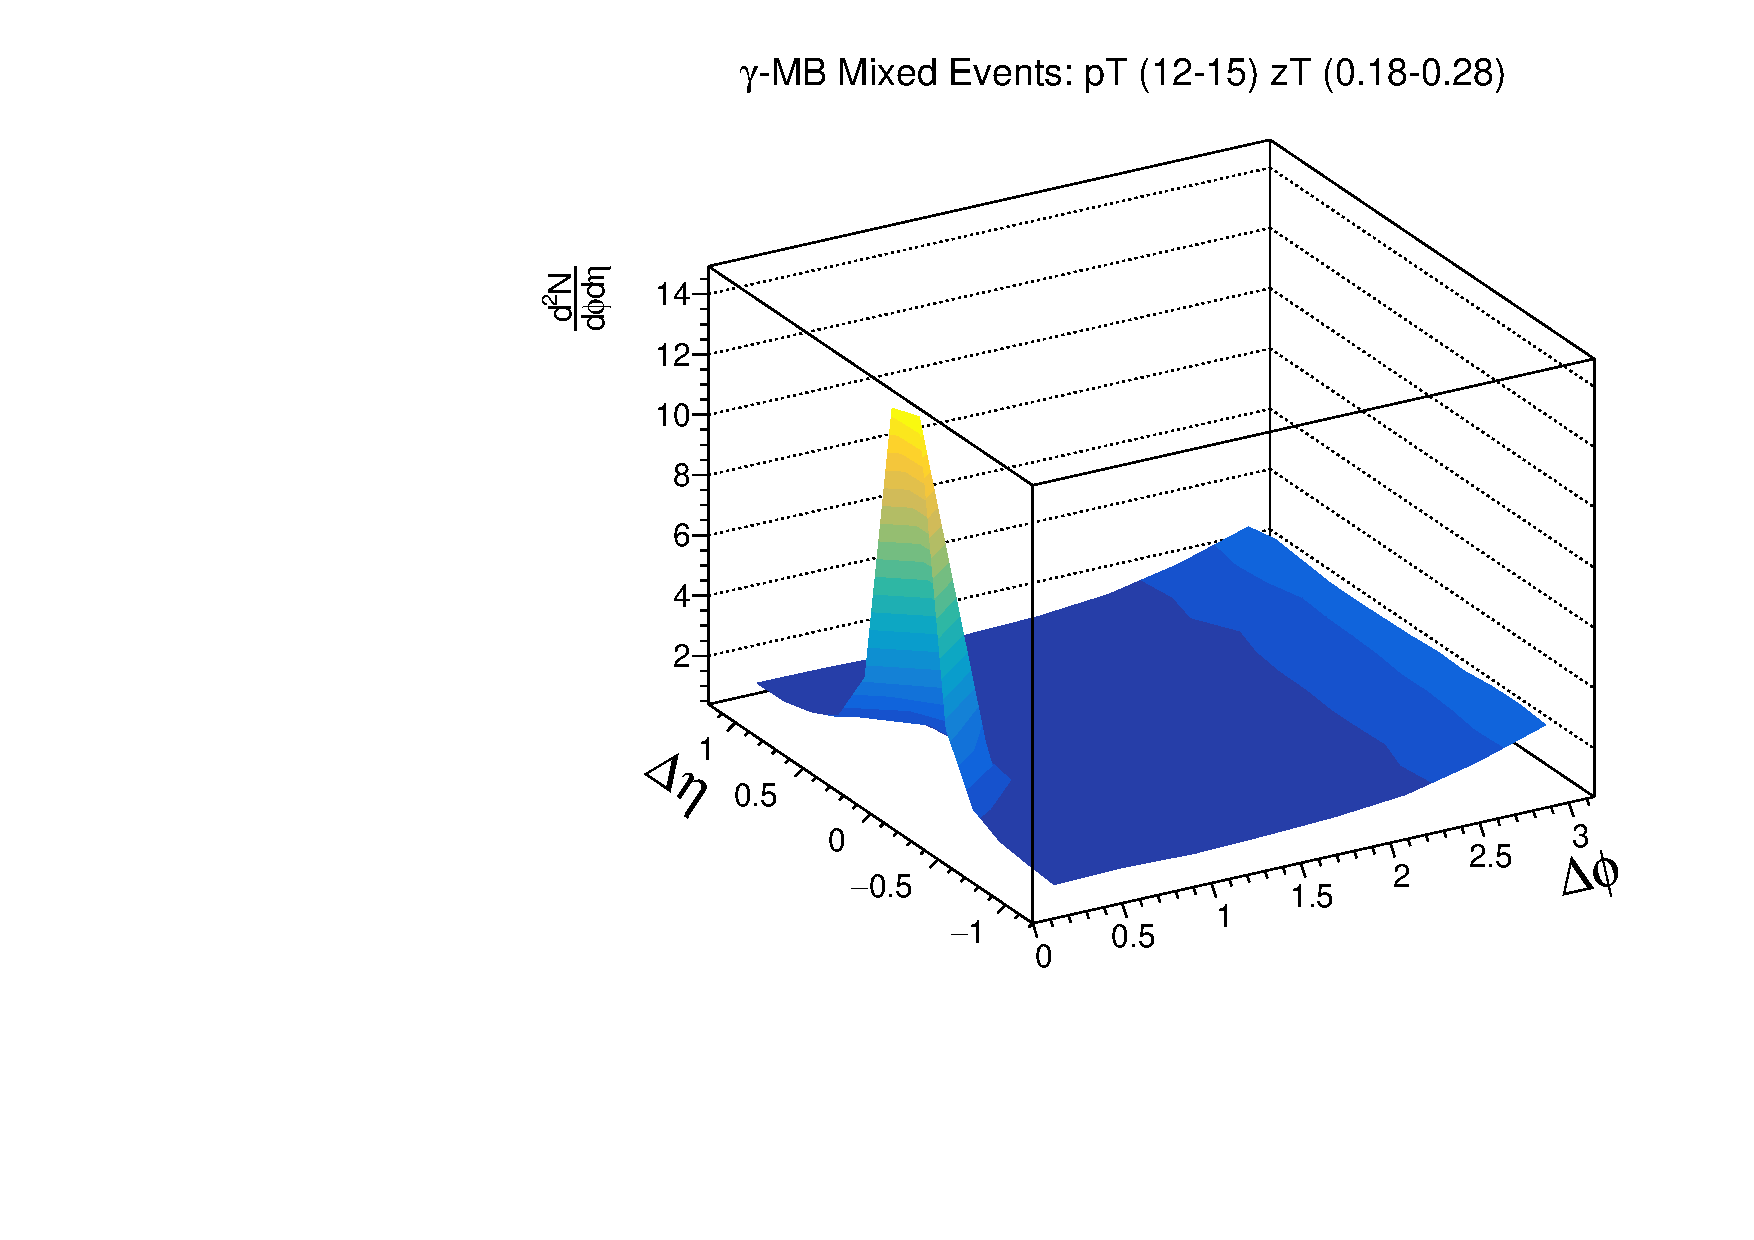
\includegraphics[width=0.49\textwidth]{EventMixing/2D_pPb_Corr.pdf}
%\includegraphics[width=0.4\textwidth]{EventMixing/13def_Eta_Inclusive.pdf}
%\caption{\textbf{Left}: Correlation function for inclusive photons, after mixed-event correction. \textbf{Right:} $\Delta\eta$ projection from $0 < \Delta\Phi <\frac{\pi}{2}$ of correlation function from a different zT bin. A flat $\Delta\eta$ projection outside of the near side peak is just one indication that detector acceptance effects are corrected for, and informs our estimate for the uncorrelated background. The correlation was normalized such that the maximum value was 1}
%\label{Same_Mix}
%\end{figure}



%\begin{figure}
%\center
%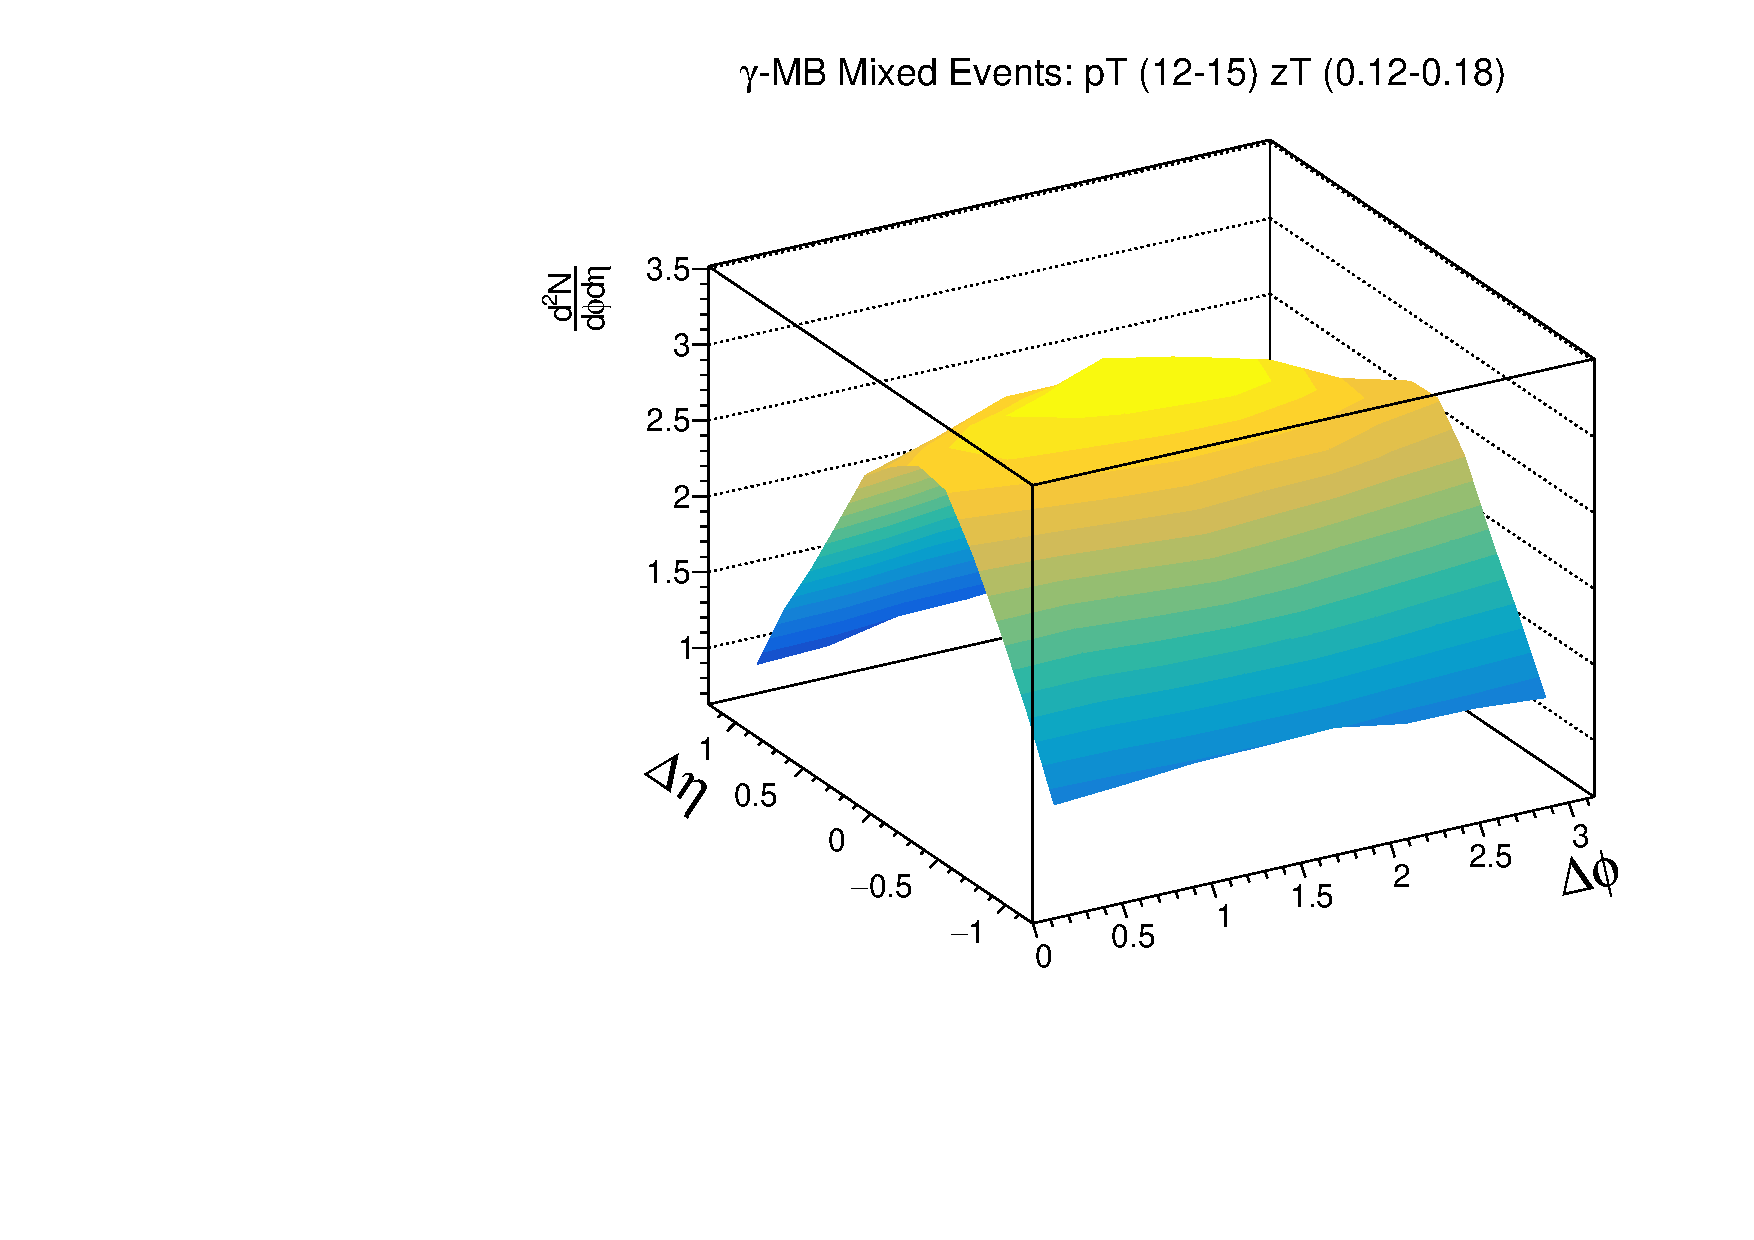
\includegraphics[width=0.7\textwidth]{EventMixing/2D_Bin_Corr.pdf}%
%\caption{10 Mixed-Event correlation using the traditional binning method. The major features presented in the Gale-Shapley-Paired Mixed event correlation are reproduced in this low-statistics binned mixing check; The trapezoidal shape in $\Delta\eta$ and the non-uniformity in $\Delta\phi$ from holes in the ITS are reproduced.}
%\label{BIN_Mixed_2D}
%\end{figure}



% At \(\Delta\phi, \Delta\eta\) = (0,0), it is assumed that the trigger and associated particle experience the same detector affects. The mixed event correlation function was therefore normalized to 1 at \(\Delta\phi \Delta\eta\) = (0,0). The overall corrected same event correlation is then given by:


%Too much detail, this is fine for your thesis but for the approval I think we should just show the results. 
%The pseudo code below follows this description, using \(\gamma\) to denote a \(\gamma\)-triggered event, and \(M_B\) to denote a minimum-bias event. The \textit{unrequested} state refers to a \(M_B\) event on a \(\gamma\)-event's preference list that has not yet been requested for pairing.\\

%\FloatBarrier
%\begin{algorithmic}
%\Procedure{GaleShapleyPairing}{}
%\While{\(\exists\) \textit{free} \(\gamma\) with an unrequested \(M_B\) on \(\gamma\)'s list}
%\State \(M_B\) = first unrequested MinBias Event on \(\gamma\)'s list.
%\If {\(M_B\) is free}
%\State (\(\gamma\),\(M_B\)) become paired
%\Else{ some pair (\(\gamma\)',\(M_B\)) exists}%
%	\If{\(M_B\) prefers \(\gamma\) to \(\gamma\)'}
%    \State \(\gamma\)' becomes free
%    \State (\(\gamma\),\(M_B\)) become paired
%    \Else
%    \State (\(\gamma\)',\(M_B\)) remain paired
%    \EndIf
%\EndIf
%\EndWhile
%\EndProcedure
%\end{algorithmic}
%\FloatBarrier

%$\epsilon$ is the single track efficiency described in section \ref{sec:Efficiency_fake_rates}, and $f$ is the fake rate given in Equation \ref{eq:fakes}

%\begin{figure}
%\center
%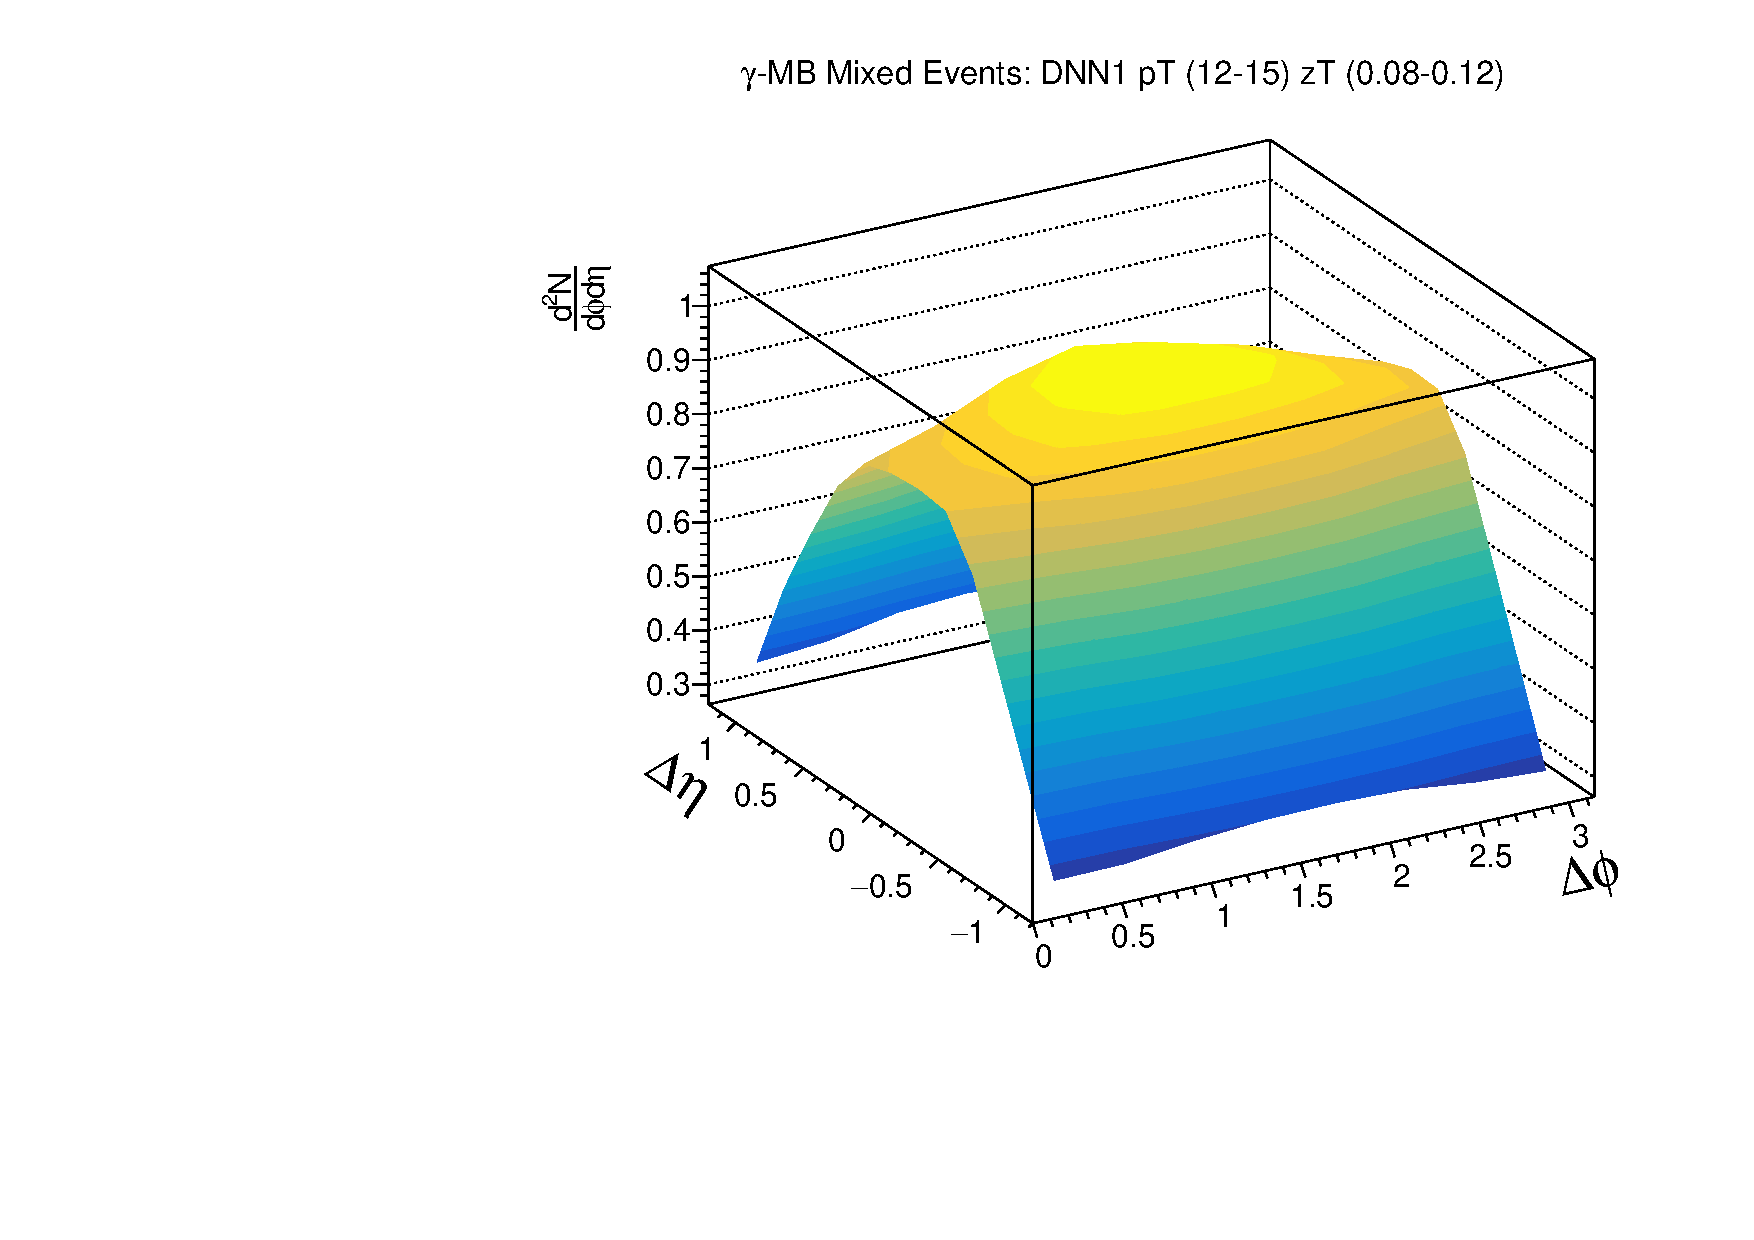
\includegraphics[width=0.495\textwidth]{EventMixing/2D_13def_signal_Correlations.pdf}
%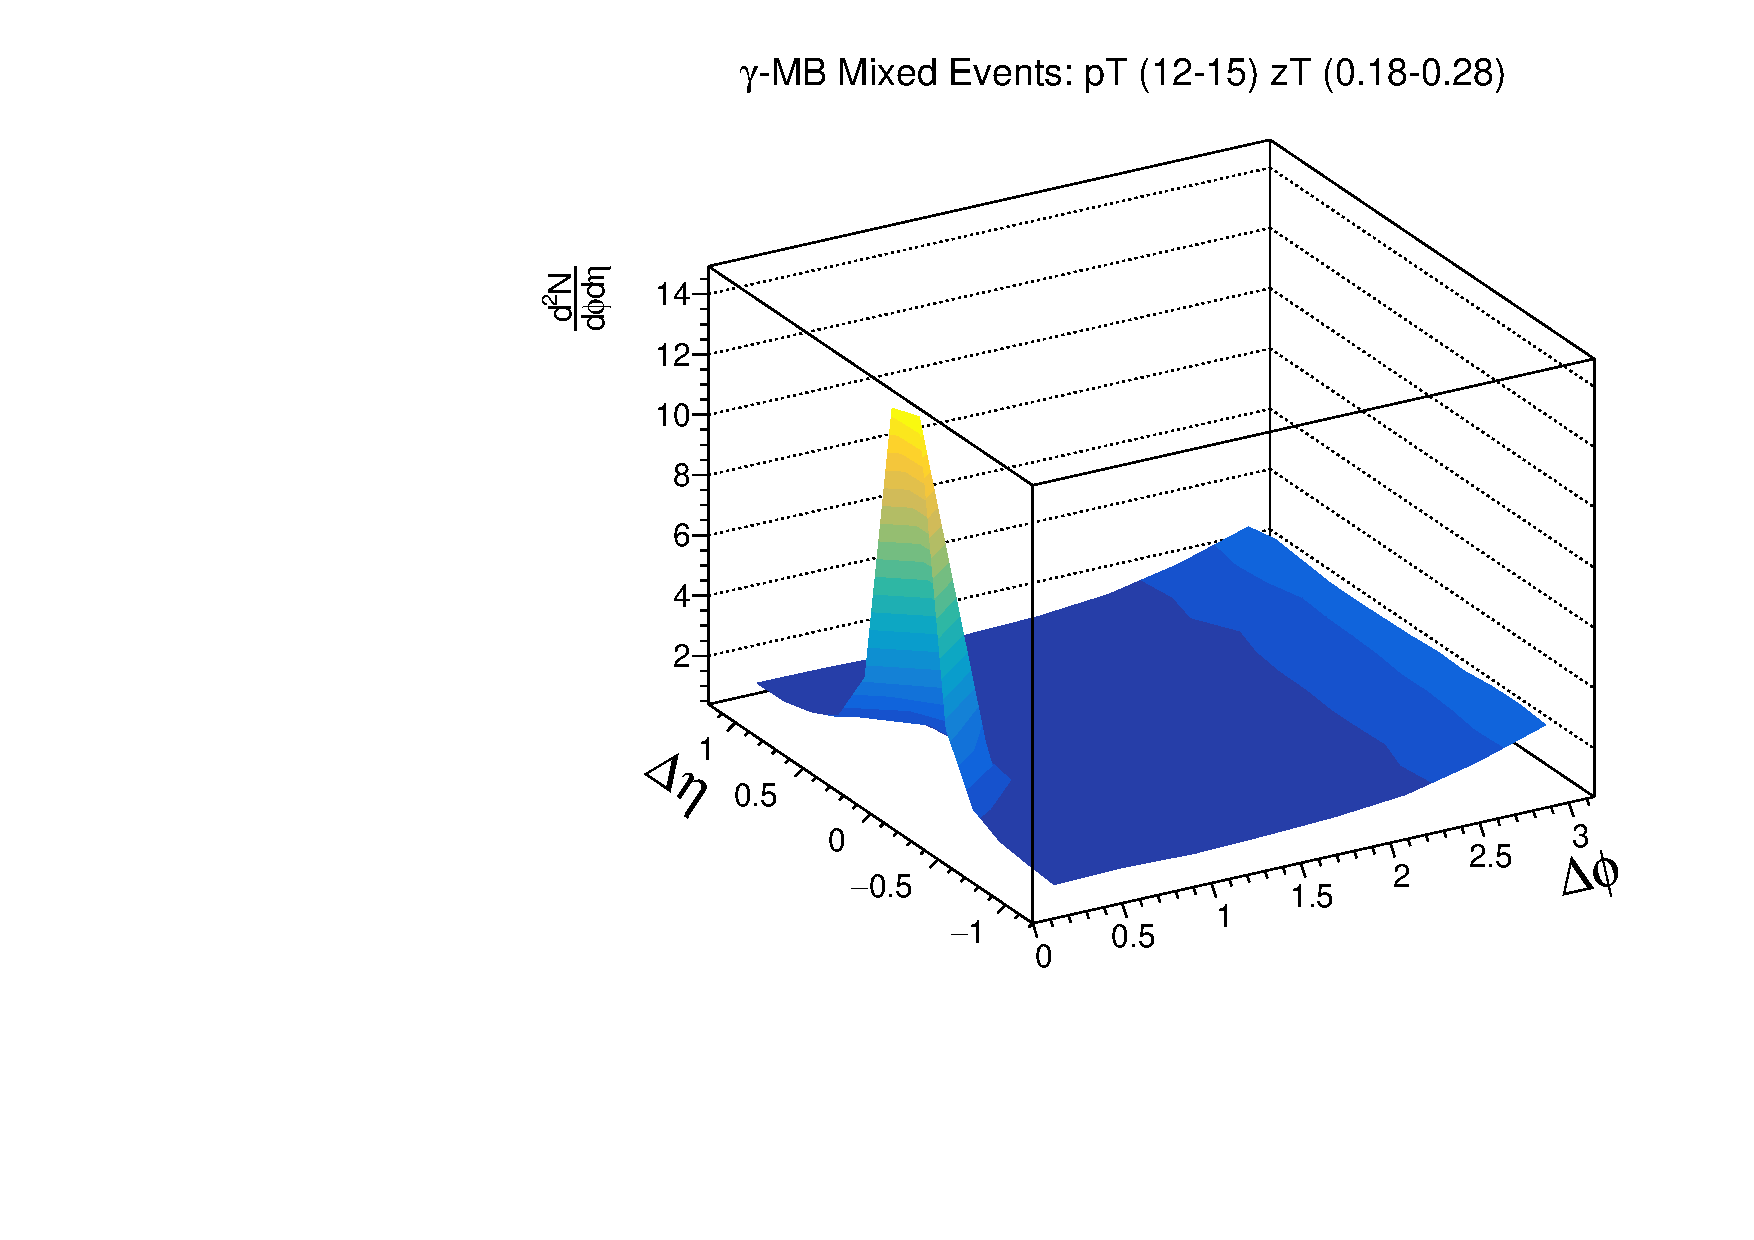
\includegraphics[width=0.495\textwidth]{EventMixing/2D_pPb_Corr.pdf}
%\caption{\textbf{Left}:Mixed event correlation for a single $z_T$ bin. The trapezoidal shape in $\Delta\eta$ is due to the convolution of EMCal and ITS acceptances in $\eta$. The non-uniformity in $\Delta\phi$ is attributed to holes in the ITS acceptance. \textbf{Right}: Correlation function for inclusive photons, after mixed-event correction.}
%\label{GS_Mixed_2D}
%\end{figure}